\documentclass[a4paper, 12pt, twoside]{article}
\usepackage[T2A,T1]{fontenc}
\usepackage[utf8]{inputenc}
\usepackage[english, russian]{babel}
\usepackage{graphicx}
\usepackage[hcentering, bindingoffset = 10mm, right = 15 mm, left = 15 mm, top=20mm, bottom = 20 mm]{geometry}
\usepackage{multirow}
\usepackage{ctable}
\usepackage{lipsum}
\usepackage{amsmath, amstext}
\usepackage{siunitx}
\usepackage{subcaption}
\usepackage{wrapfig}
\usepackage{adjustbox}
\usepackage{enumerate, indentfirst, float}
\usepackage{capt-of, svg}
\usepackage{cmap} % Улучшенный поиск русских слов в полученном pdf-файле

\usepackage{pscyr} % Нормальные шрифты
\usepackage[normalem]{ulem} % для подчёркиваний uline
\ULdepth = 0.16em
%% Перенос знаков в формулах (по Львовскому)
\newcommand*{\hm}[1]{#1\nobreak\discretionary{}
	{\hbox{$\mathsurround=0pt #1$}}{}}

\usepackage{fancyhdr} %Колонтикулы
\pagestyle{fancy}
\lhead{
\includegraphics[width = 10 mm]{logo.jpg} Применения операционных усилителей.}
\rhead{\textit{\today}}

\newenvironment{bottompar}{\par\vspace*{\fill}}{\clearpage}
 
\begin{document}
\begin{titlepage}

\newcommand{\HRule}{\rule{\linewidth}{0.7mm}} % Defines a new command for the horizontal lines, change thickness here

\center % Center everything on the page
 
%----------------------------------------------------------------------------------------
%	HEADING SECTIONS
%----------------------------------------------------------------------------------------

\textsc{\LARGE Московский Физико-Технический Институт}\\[1,5cm] % Name of your university/college

\textsc{\large Лабораторная работа по радиотехническим сигналам и цепям}\\[0.5cm] % Minor heading such as course title

%----------------------------------------------------------------------------------------
%	TITLE SECTION
%----------------------------------------------------------------------------------------

\HRule
\\[0.4cm]
{ \huge \bfseries Применение операционных усилителей.}
\\[0.4cm] % Title of your document
\HRule
\\[1.5cm]


 
%----------------------------------------------------------------------------------------
%	AUTHOR SECTION
%----------------------------------------------------------------------------------------


	\begin{center} \large
		\textbf{Автор:}\\
		Глеб Уваркин \\
		615 группа
	\end{center}

~


\begin{bottompar}
	\begin{center}
		
\includegraphics[width = 80 mm]{logo.jpg}
	\end{center}
	{\large \today}

\end{bottompar}
\vfill % Fill the rest of the page with whitespace

\end{titlepage}

\section*{Задание №1.Измерение коэффициента усиления ОУ.}

\begin{figure}[H]
	\centering
	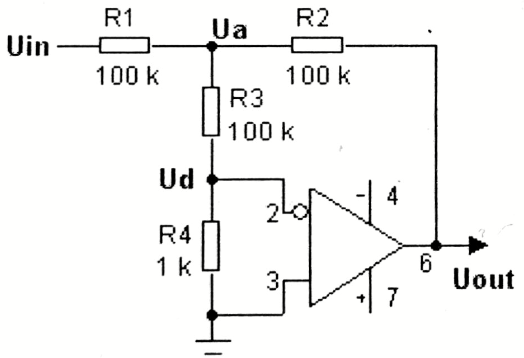
\includegraphics[width =  0.3\linewidth]{kus}
	\caption{Схема измерения коэффициента усиления.}
	\label{kus}

\end{figure}


Соберём схему, показанную на рис. \ref{kus}. Сопротивления резисторов возьмём: $R_1=R_2=R_3=200$ кОм, $R_4 = 2$ кОм, $R_3/R_4 = 100$.
\vspace{\baselineskip}

Подадим на вход колебание с амплитудой $U_{in} = 2.5$ В и частотой $f = 15$ Гц. Измерим величину напряжений $U_a$ и $U_{out}$: $U_a = 4.4 $ мВ, $U_{out} = 2.46$ В. 

\vspace{\baselineskip}

Рассчитаем коэффициент усиления операционного усилителя по формуле $A_0 = (1 \hm{+}R_3/R_4)\cdot (U_{out}/U_a)$:
$$A_0 = (1 + 100)\dfrac{2.46}{4.4\cdot 10^{-3}} = 56468  \simeq 6 \cdot 10^4$$.

\section*{Задание №2. Амплитудно-частотная характеристика ОУ.}

Для схемы на рис. \ref{kus} снимем зависимость коэффициента усиления от частоты (АЧХ), используя формулу: $$A(f) = \dfrac{U_{out}}{U_d} = \dfrac{U_{out}}{U_a}\cdot \dfrac{U_a}{U_d} = \left(1+\dfrac{R_3}{R_4}\right )\cdot \dfrac{U_{out}}{U_a}.$$
Занесём полученные данные в таблицу \ref{kus}.

\begin{table}[H]
	\centering
	\caption{Зависимость коэффициента усиления от частоты.}
	\label{kus}
	\begin{tabular}{c|c|c|c|c|c|c|c|c|c|c}
		\toprule
		$f,$ Гц      & 50    & 100   & 200   & 500  & 1000 & 2000 & 5000 & 10000 & 20000 & 50000 \\ 
		$U_{out},$ В & 2.48  & 2.48  & 2.48  & 2.48 & 2.47 & 2.43 & 2.21 & 1.73  & 1.06  & 0.76  \\ 
		$U_a,$ мВ    & 5.55  & 8.67  & 16    & 39   & 77   & 152  & 343  & 543   & 131   & 119   \\ 
		$A$          & 45000 & 29000 & 16000 & 6000 & 3000 & 1600 & 651  & 324   & 82    & 65    \\ \midrule
		$lgf$        & 1.7   & 2     & 2.3   & 2.7  & 3    & 3.3  & 3.7  & 4     & 4.3   & 4.7   \\ 
		$20lgA,$ дБ      & 93    & 89    & 84    & 76   & 69   & 64   & 56   & 50    & 38    & 36    \\ \bottomrule
	\end{tabular}
\end{table}

Построим снятую зависимость в двойном логарифмическом масштабе, откладывая частоту в герцах, а коэффициент усиления в децибелах.

\begin{figure}[H]
	\centering
	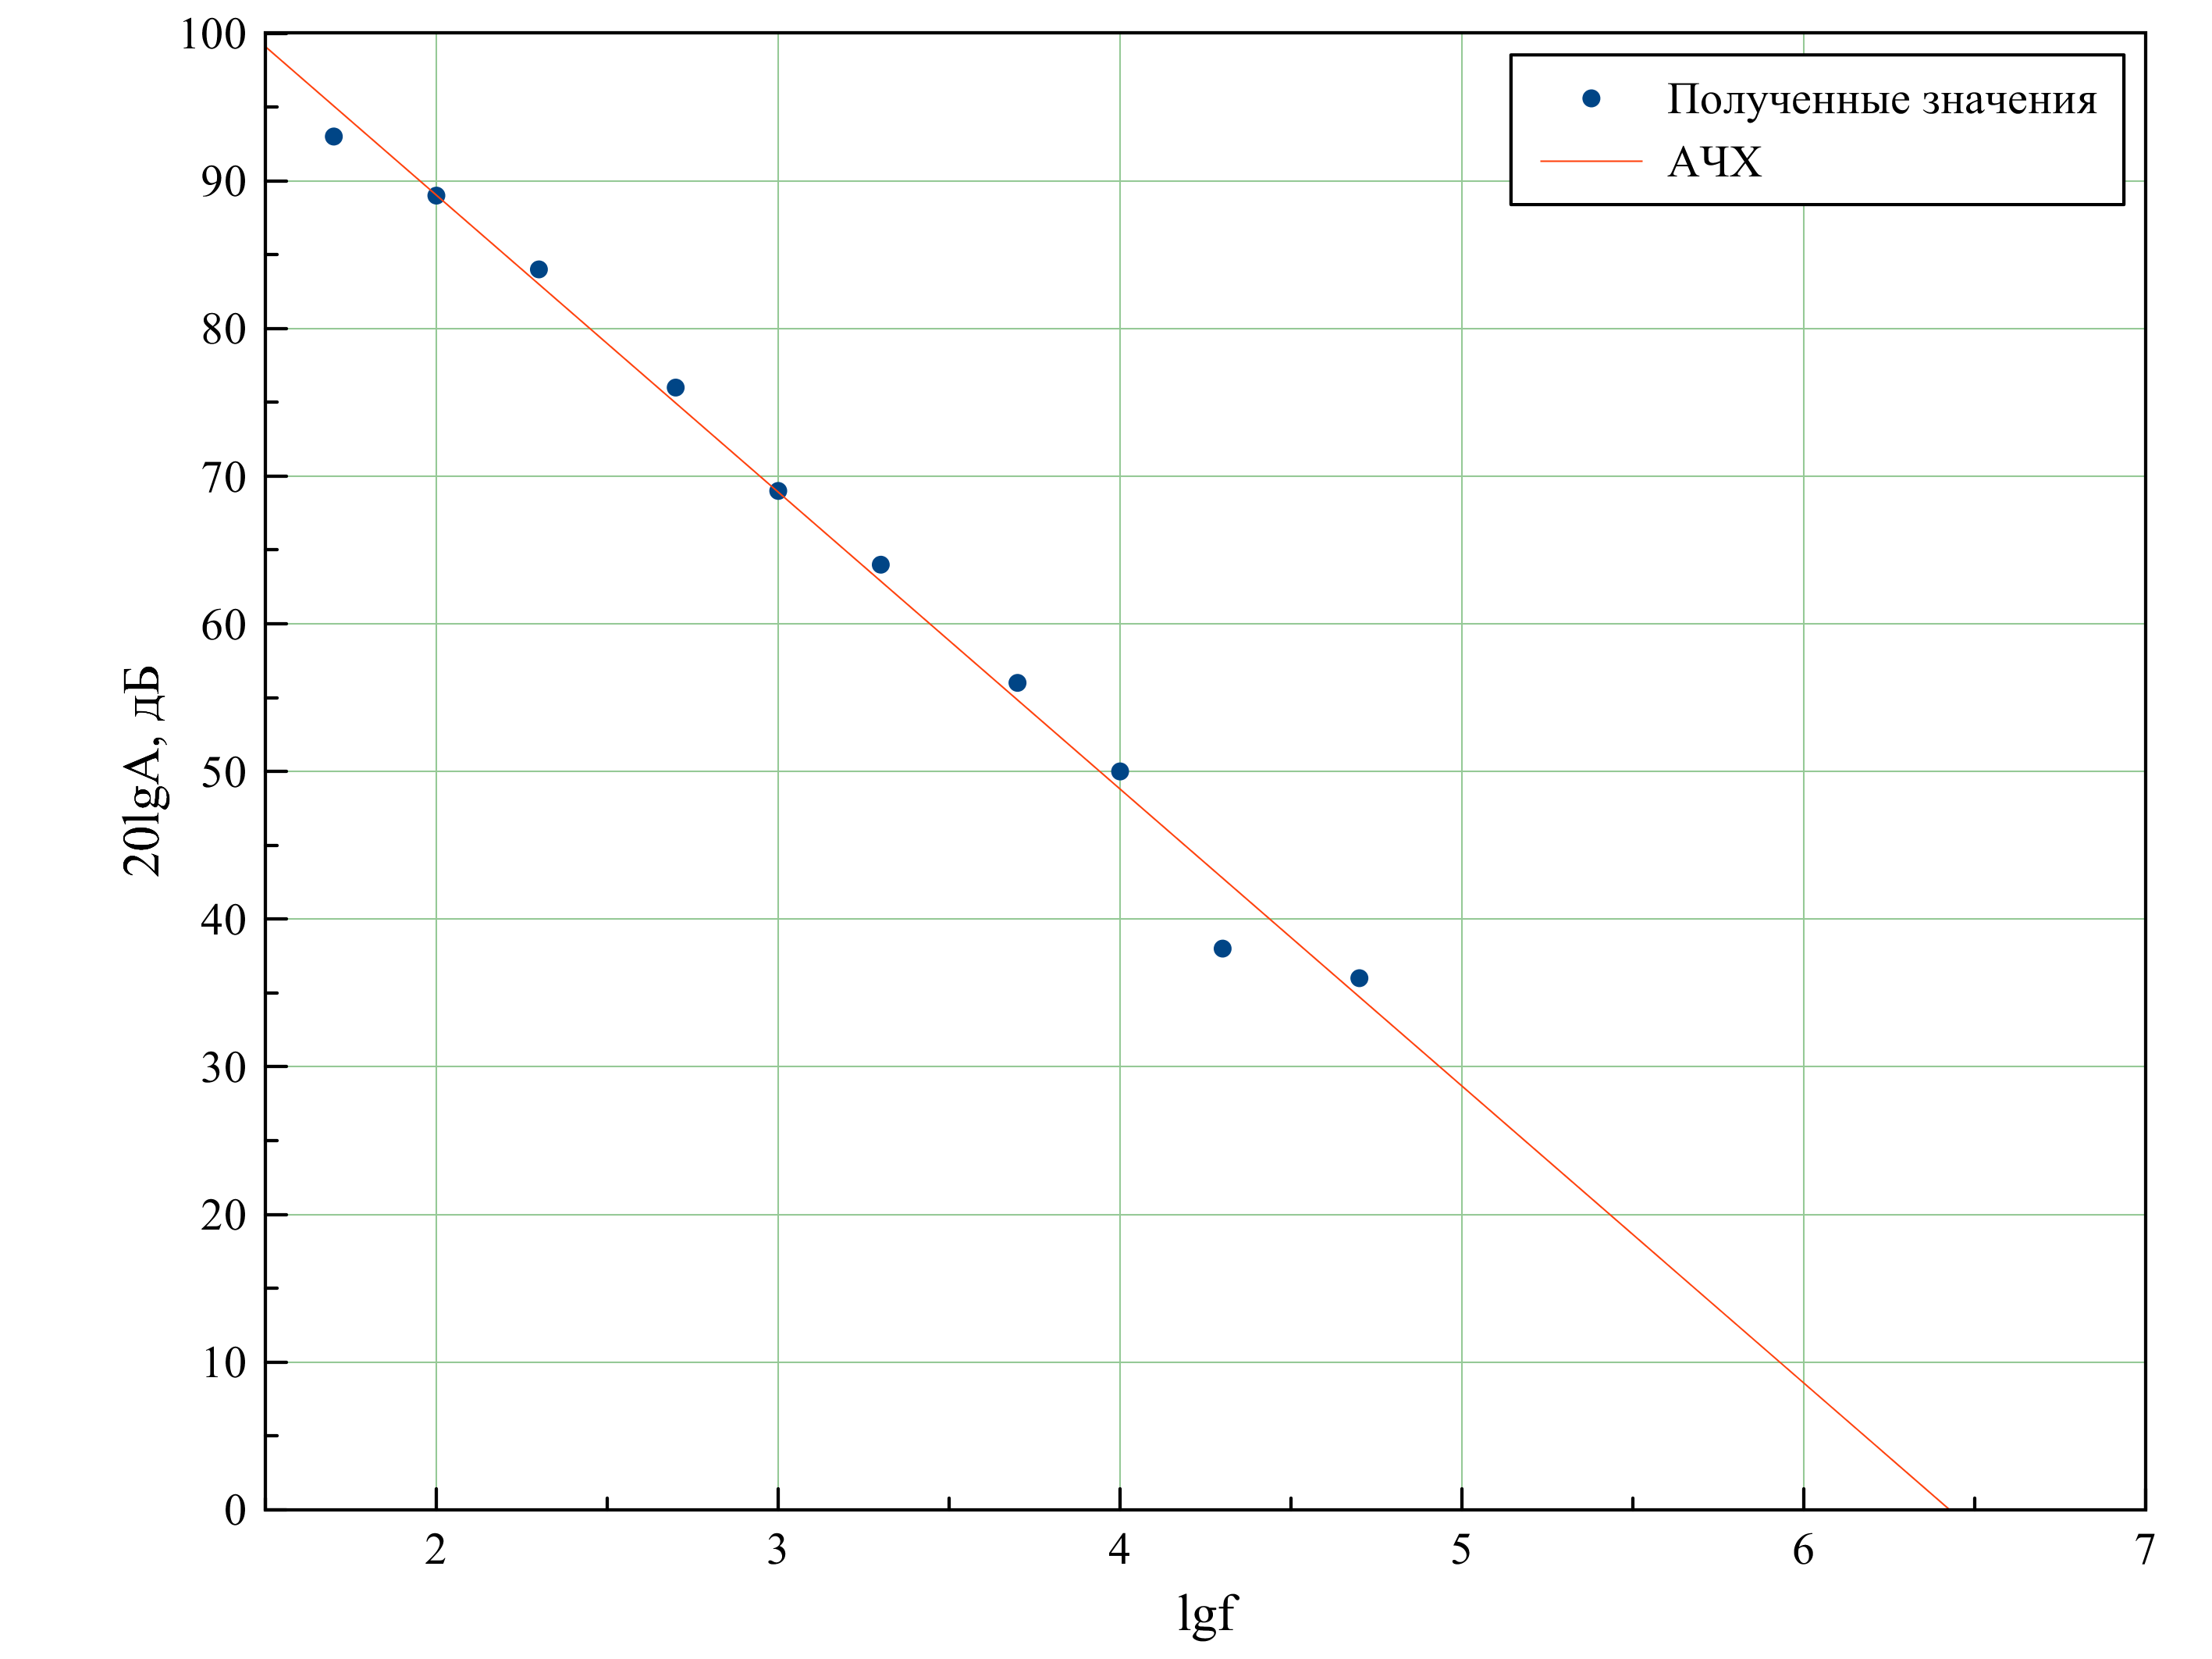
\includegraphics[width =  0.8\linewidth]{1}
	\caption{ АЧХ ОУ.}
	\label{ACHX}
\end{figure}

Из  рис. \ref{ACHX} получаем следующие величины:
$$f_T \simeq 3~ \text{МГц}, f_{p_0} \simeq 45~ \text{кГц} $$.
На частотах $f > f_{p_0}$ усиление падает обратно пропорционально частоте - с крутизной спада $-20$ дб/декада.

\section*{Задание №3. Неинвертирующий усилитель.}

\begin{figure}[H]
	\centering
	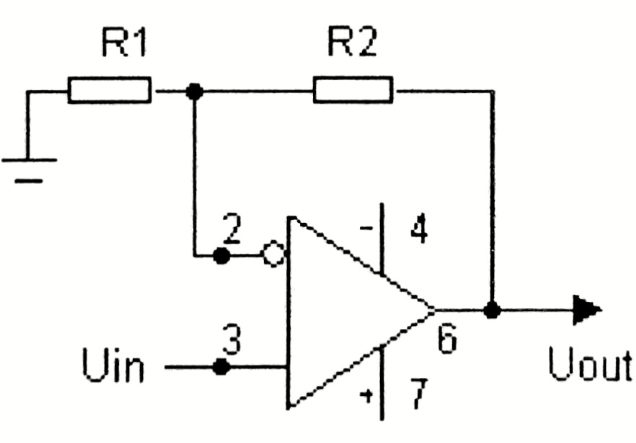
\includegraphics[width =  0.3\linewidth]{nus}
	\caption{Схема неинвертирующего усилителя.}
	\label{nus}
\end{figure}

Соберём схему, возьмём $R_1 = 2$ кОм, $R_2 = 200$ кОм, $R_2/R_1 = 100$.
\vspace{\baselineskip}

Измерим постоянное напряжение на выходе $U_{out(dc)} \simeq 68$ мВ. Определим входное напряжение сдвига ОУ: $U_{OS} = U_{out(dc)}/(1+R_2/R_1).$ Получим $U_{OS} \simeq 68/(1 + 100)\simeq 673$ мкВ.
\vspace{\baselineskip}

Снимем зависимость от частоты коэффициента усиления $K(f)$ при $U_{\text{вх}} = 10$ мВ. Полученные данные занесём в таблицу \ref{kust}.

\begin{table}[H]
	\centering
	\caption{Зависимость коэффициента усиления $K(f)$.}
	\label{kust}
	\resizebox{\textwidth}{!}{%
	\begin{tabular}{c|c|c|c|c|c|c|c|c|c|c|c|c|c|c|c}
		\toprule
		$f,$ Гц             & 50   & 100  & 200  & 500  & 1k   & 2k   & 5k   & 10k  & 20k & 50k  & 100k & 150k & 300k & 500k & 1M   \\ 
		$U_{\text{вых}},$ В & 1.04 & 1.04 & 1.04 & 1.04 & 1.04 & 1.03 & 1.02 & 0.97 & 0.9 & 0.55 & 0.31 & 0.21 & 0.11 & 0.07 & 0.03 \\ 
		K                   & 104  & 104  & 104  & 104  & 104  & 103  & 102  & 97   & 90  & 55   & 31   & 21   & 11   & 7    & 3    \\ \bottomrule
	\end{tabular}%
}
\end{table}

\begin{figure}[H]
	\centering
	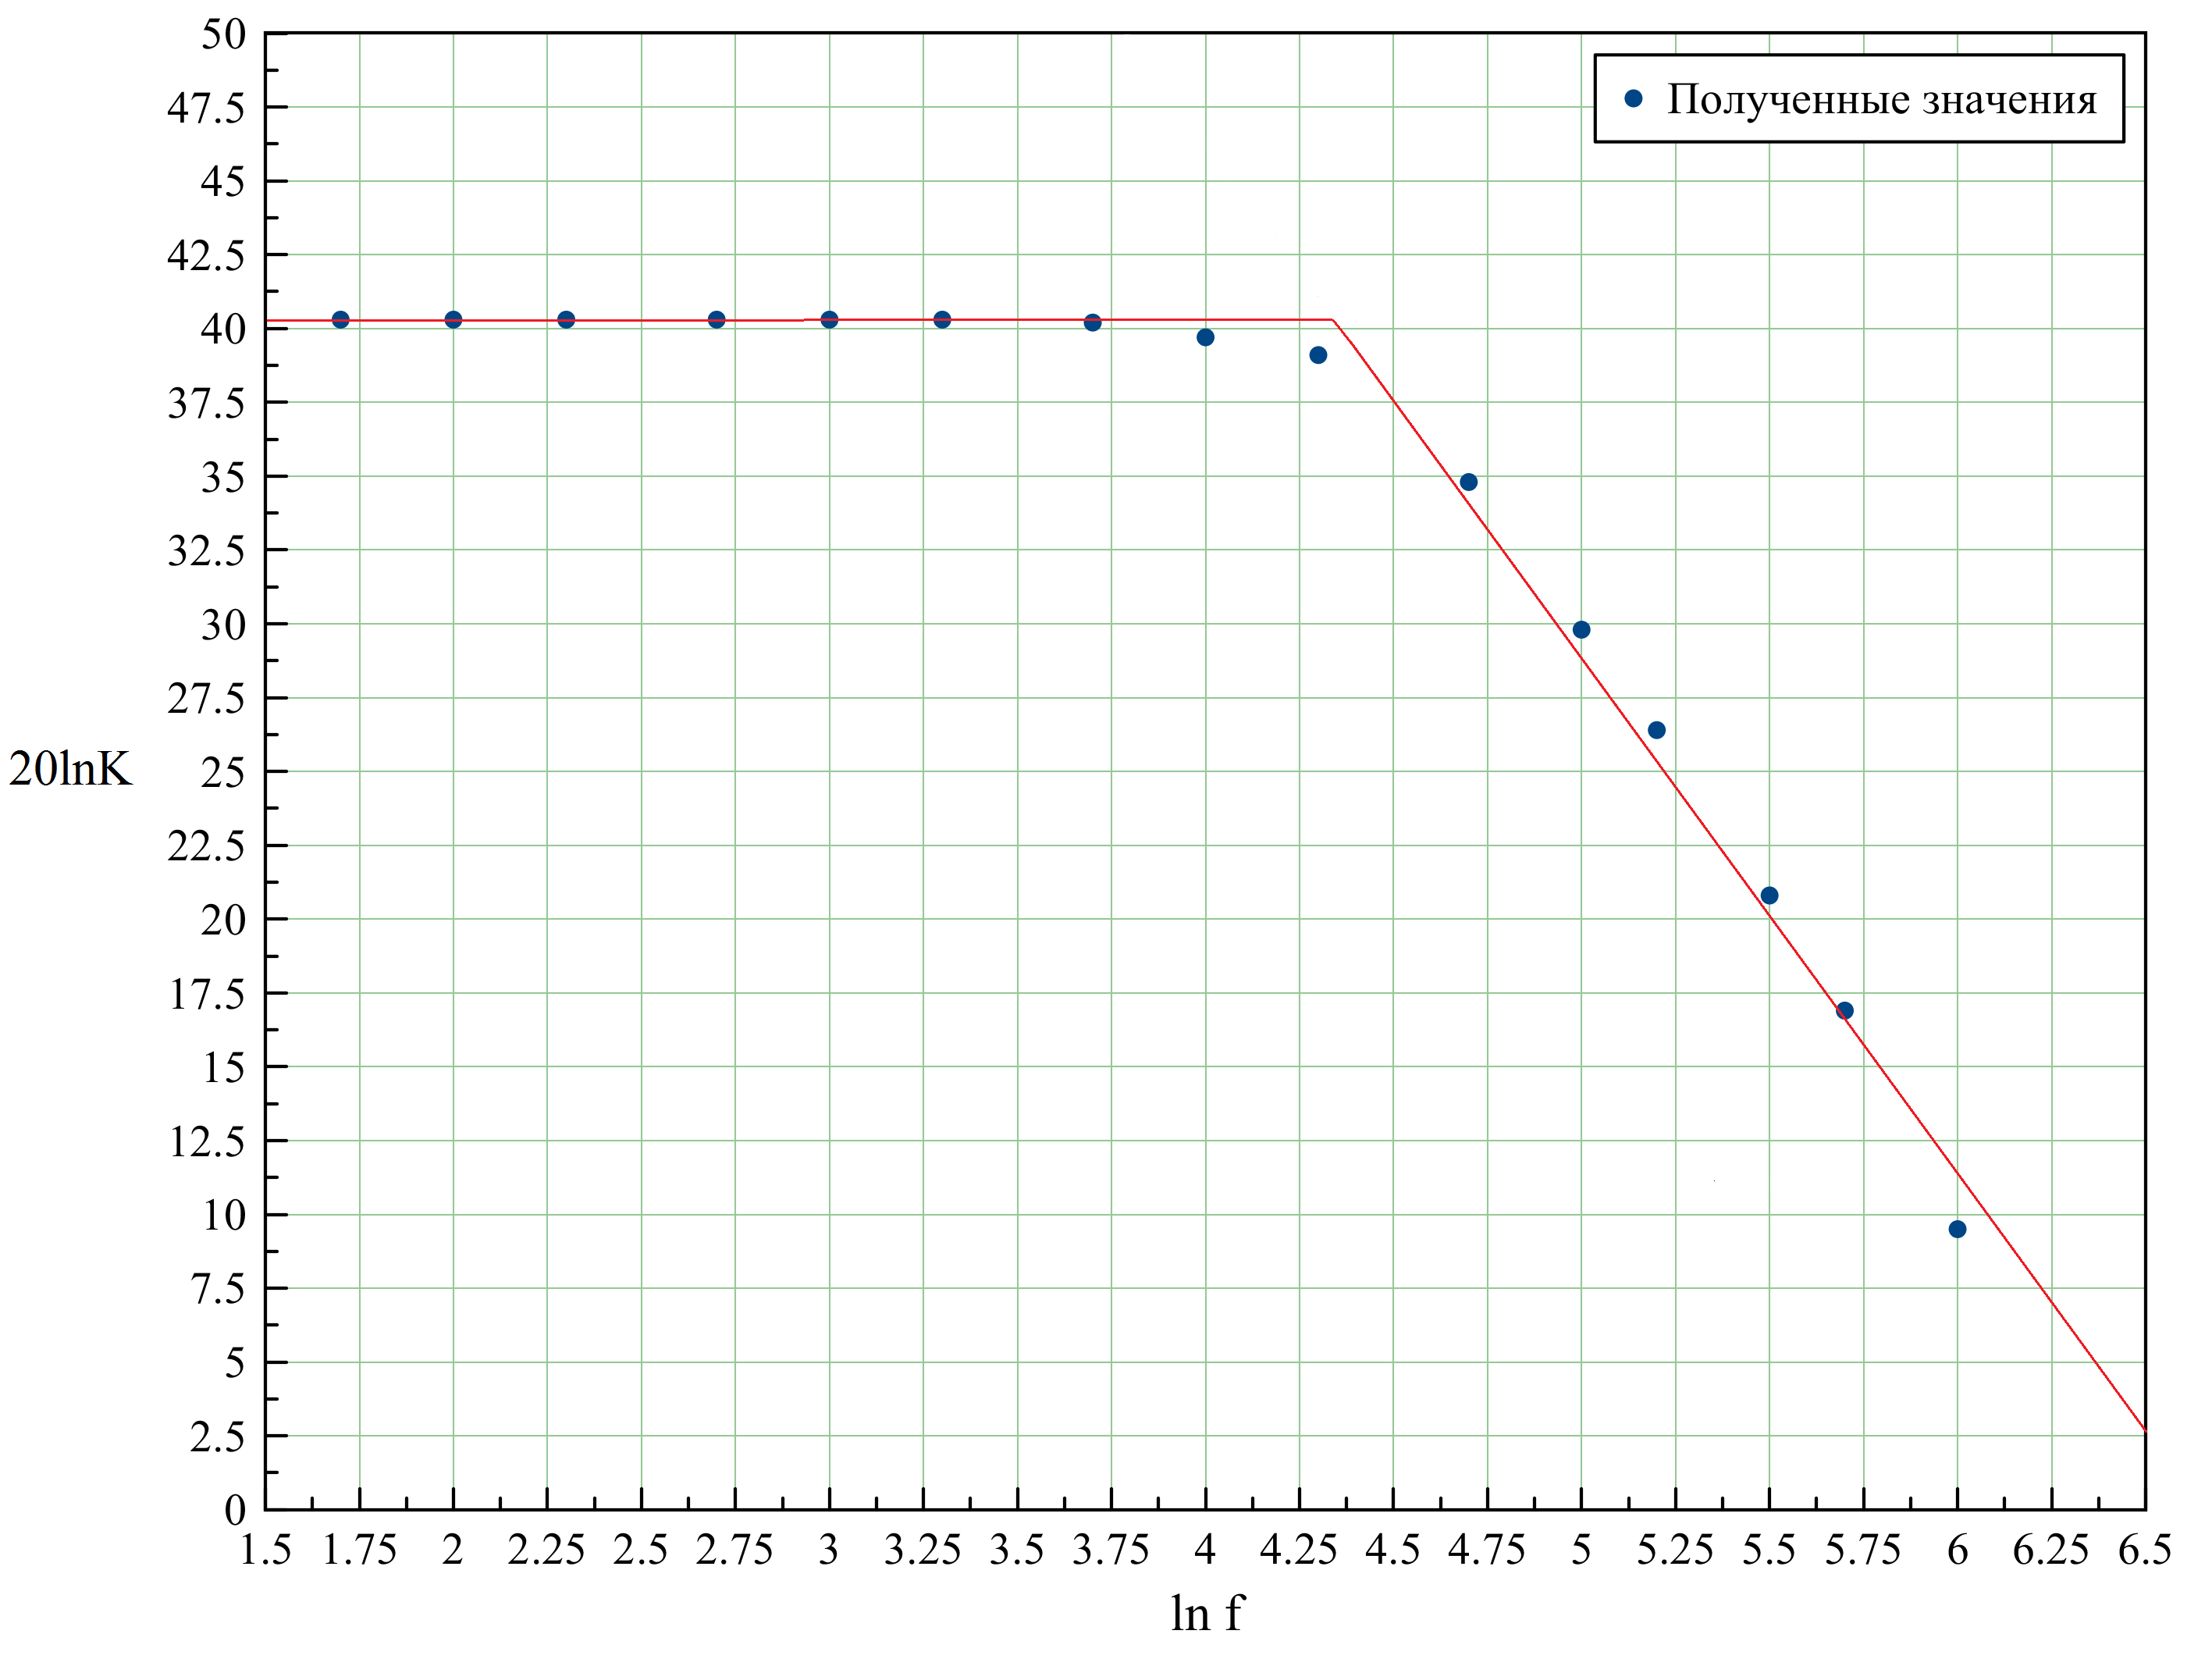
\includegraphics[width =  0.7\linewidth]{3}
	\caption{Зависимость коэффициента усиления $K(f)$.}
	\label{kf}
\end{figure}

Из рис. \ref{kf} определим граничную частоту $F_p$ по уровню $0.7$ относительно коэффициента усиления на низких частотах. Получим $F_p \simeq 31.6$ кГц.
\vspace{\baselineskip}

Проверим, что коэффициент усиления на низких частотах ($f < F_p$) и граничная частота усилителя удовлетворяет соотношениям: $K_0 = 1/\beta = 1+R_2/R_1;~ F_p = \beta f_T,~ \beta \hm{=} R_1/(R_1+R_2)$ - коэффициент отрицательной обратной связи.

$$\beta = 2/(2+200) \simeq 0.01 $$  
$$K_0 = 1/0.01 = 100 \simeq 101 = 1 + 200/2$$
$$31.6 \cdot 10^3 \simeq 0.01\cdot 3 \cdot 10^6$$

Все соотношения выполняются.
\vspace{\baselineskip}

Определим максимальную амплитуду неискажённого выходного напряжения на низкой частоте $f = 1.5$ кГц. Получим $U_{\text{вых}} \simeq 3.2$ В.
\vspace{\baselineskip}

Включим ОУ по схеме повторителя ($R_1 = \infty,~R_2 = 0$). Измерим коэффициент передачи и граничную частоту усилителя. Определим на частоте $f = 0.8$ МГц максимальную амплитуду неискажённого сигнала и характер искажений, возникающих при дальнейшем увеличении амплитуды входного сигнала. Получим $U_{m\_out} \simeq 3.0$ В. ("скошенная синусоида").
\begin{table}[H]
	\centering
	\caption{Зависимость коэффициента передачи повторителя.}
	\label{zk}
	\resizebox{\textwidth}{!}{%
	\begin{tabular}{c|c|c|c|c|c|c|c|c|c|c|c|c|c|c|c|c}
		\toprule
		$f,$ Гц             & 50   & 100  & 200  & 500  & 1k   & 2k   & 5k   & 10k  & 20k  & 1M   & 2M   & 2.5M & 2.6M & 3.4M & 5M   & 10M  \\ 
		$U_{\text{вых}},$ В & 1.00 & 1.00 & 1.00 & 1.00 & 1.00 & 1.00 & 1.00 & 1.00 & 0.98 & 1.00 & 1.05 & 1.00 & 1.00 & 0.99 & 0.60 & 0.31 \\ 
		K                   & 1.00 & 1.00 & 1.00 & 1.00 & 1.00 & 1.00 & 1.00 & 1.00 & 0.98 & 1.00 & 1.05 & 1.00 & 1.00 & 0.99 & 0.60 & 0.31 \\ \bottomrule
	\end{tabular}%
	}
\end{table}

\begin{figure}[H]
	\centering
	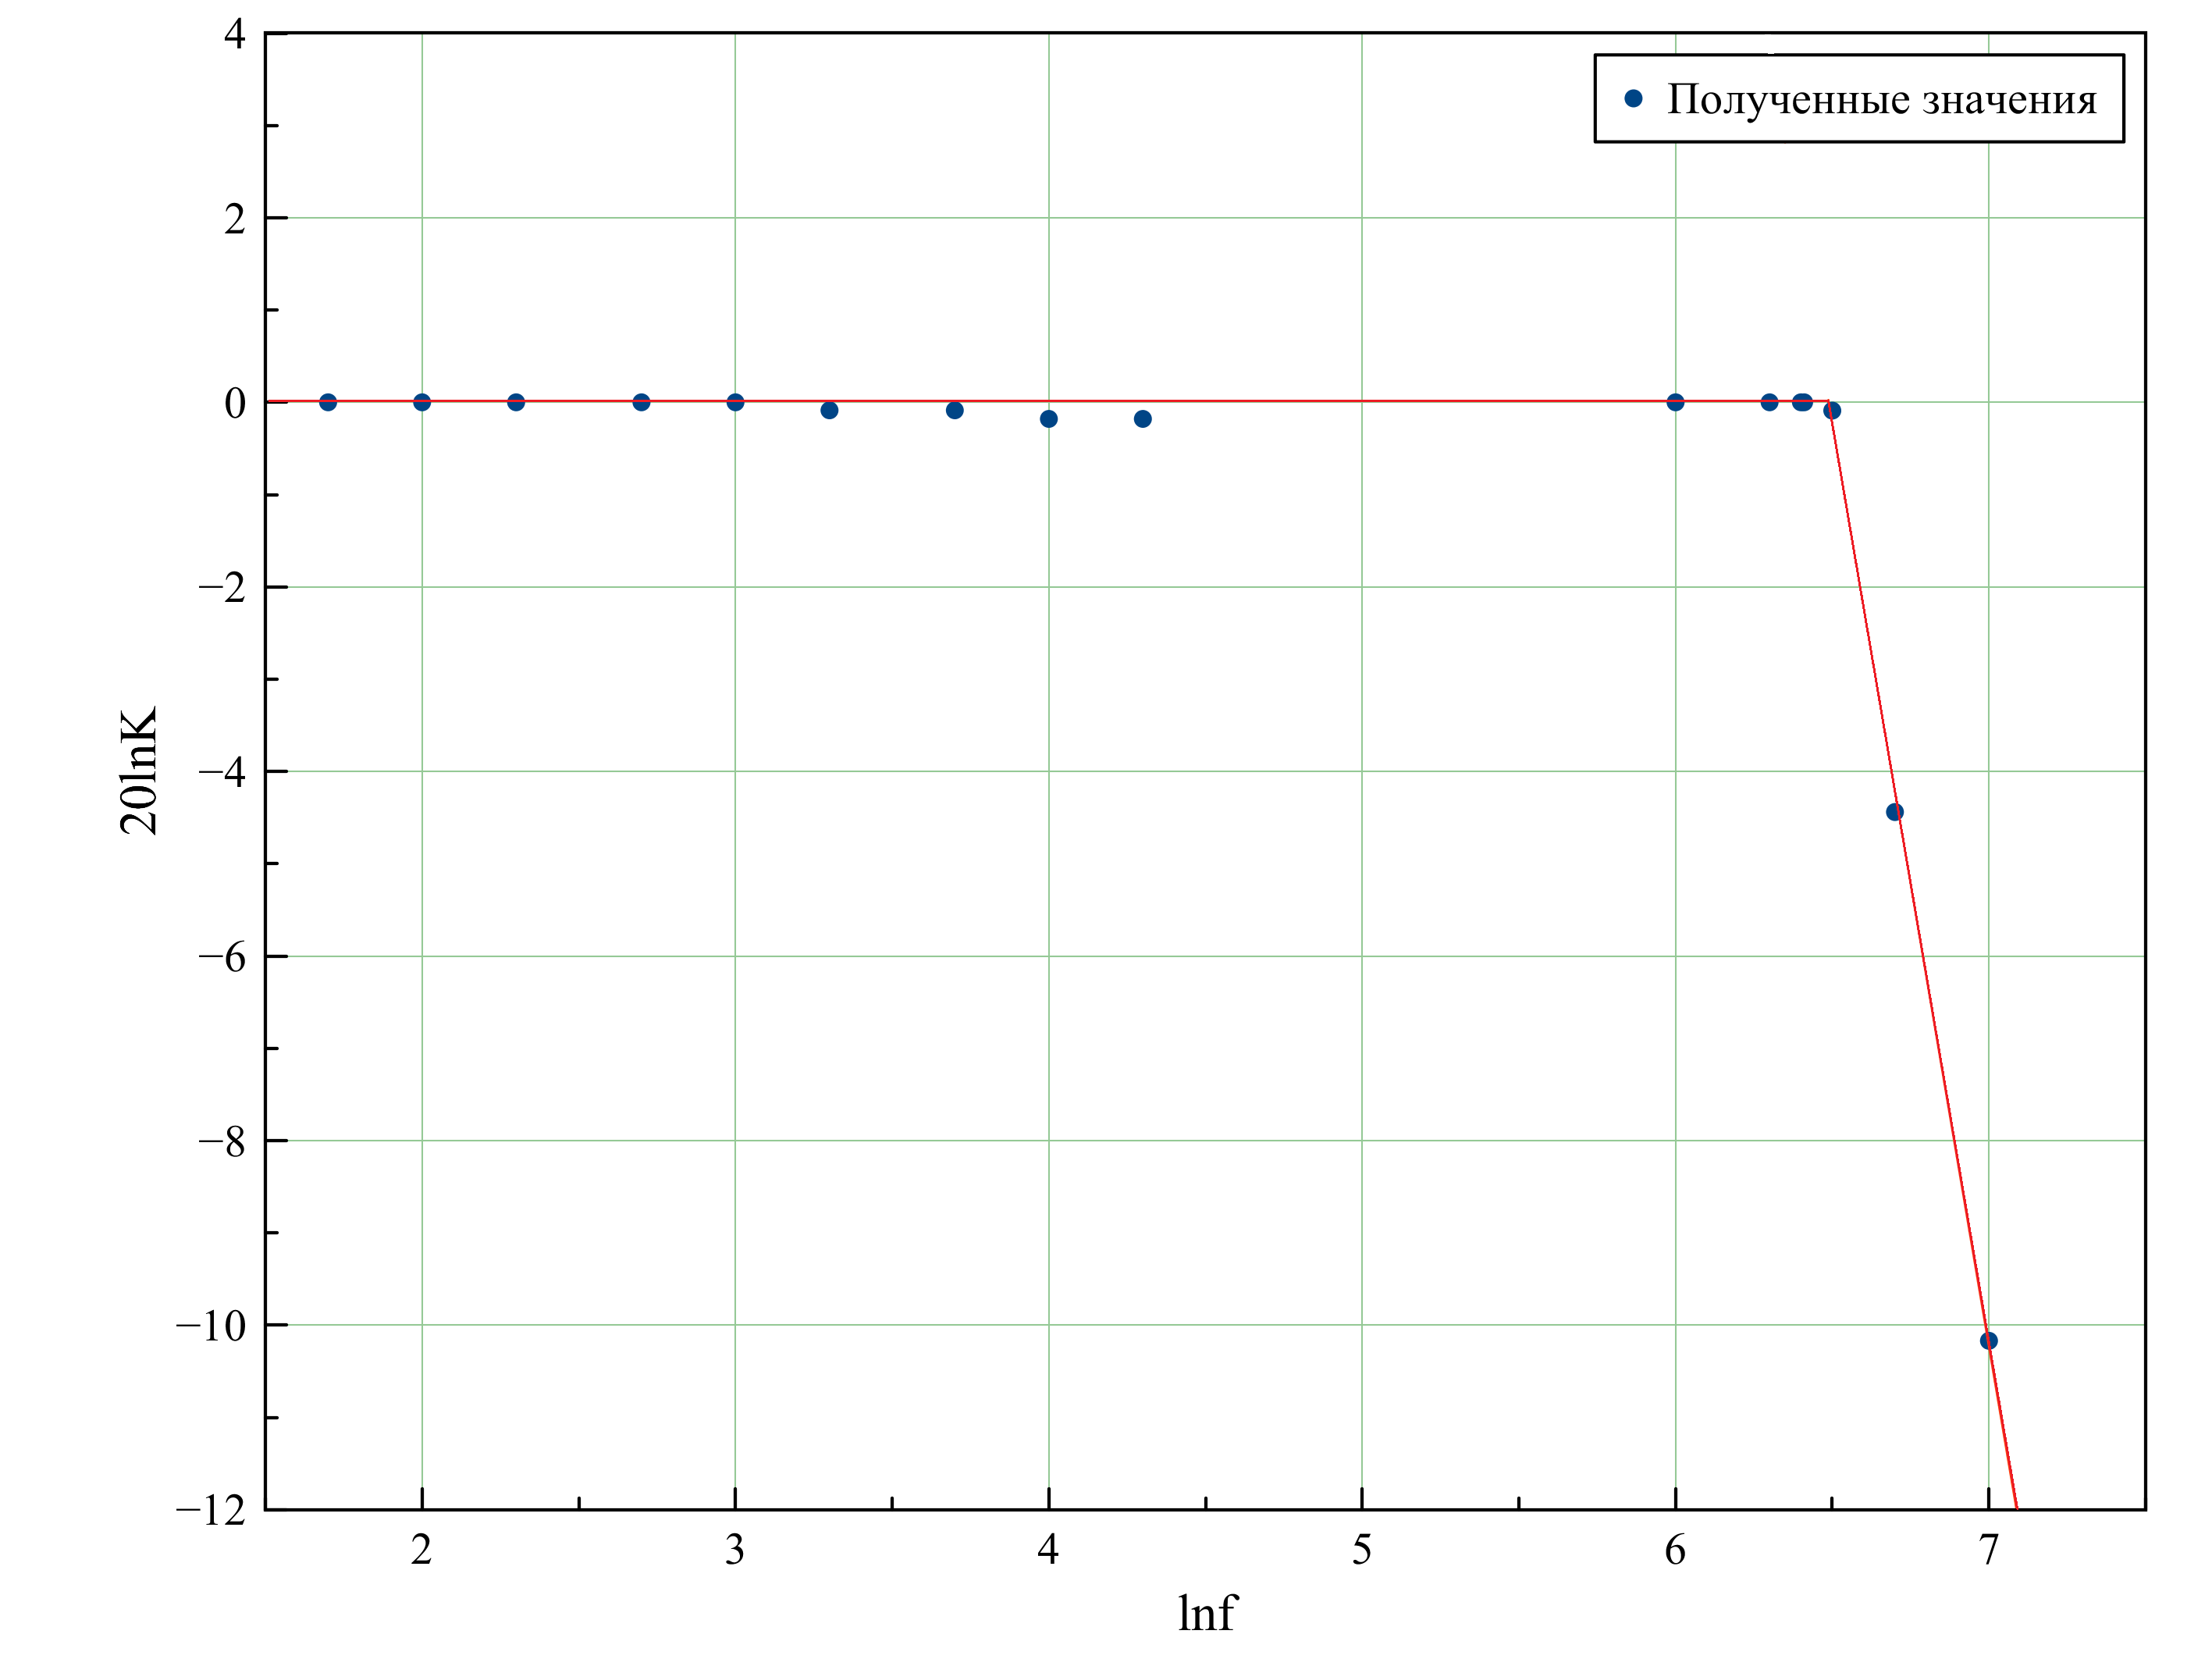
\includegraphics[width =  0.7\linewidth]{31}
	\caption{Зависимость коэффициента усиления $K(f)$ повторителя.}
	\label{kfp}
\end{figure}

Из рис. (\ref{kfp}) получаем, что граничная частота равна $f \simeq 3$ МГц.
\vspace{\baselineskip}

Сравним результат измерения максимальной амплитуды неискажённого сигнала с расчётом по формуле $U_{m\_out} = V_{max}/2\pi f$.
\vspace{\baselineskip}

$$ U_{m\_out} = \dfrac{ 13\cdot 10^6}{2\pi \cdot 0.8 \cdot 10^6} \simeq  2.6~\text{В} \approx 3.0 ~ \text{В}$$ 

\section*{Задание №4. Инвертирующий усилитель.}




\end{document}
